\section{Applying Baum Welch to Rainfall data}

\subsection{Building the Observation Matrix}

To be able to use Baum-Welch we require an observation probability matrix **ref**, thus in order to use it we must create one. To create a finite matrix of probabilities we require our data to be split into finite groups. Fortuantely the algorithm is increases in computation cost linearly with the dimensions of the observation matrix rather than squared as it does with the number of states. Through efficient implementation working with large observation matrices is feasible.

Through looking at the datasets, we can see the maximum rainfall is usually up to 1000mm. In our case this value was 743. Furthermore, the maximum precision of our data is integers. Thus, we can discretise our observations into integers up to the maximum rainfall for the given dataset. As we know from **ref**, the rows of the observation matrix represent the states and the columns represent the observations, giving us a matrix 3 by M matrix, where M is the number of observations.

We can now apply Baum-Welch to produce a HMM model that simulates integer values of daily rainfall in mm up to a given maximum amount. Code files can be found in "Baum Welch" folder under "MyCode". 

\begin{note}
    The values of the alpha and beta helper functions become extremly small for large sequence of observations. In our testing we found after about 1500 observations these values become too precise to store in "long double". This mathetmatically holds as the sum of the final alphas and betas represents the probability of observring the sequence **ref**, with a larger sequence the probability naturally decreases. We avoid this problem by using a sequence of 1000 observations. 
    
    When using this method, one must ensure the alpha and beta values are not all being stored as zeros.
\end{note}


\subsection{Local optimum vs global Optimum}

Once again from **ref**, we know that Baum-Welch converges to local optima. This suggests there may be a supperior optima, a superior fit for the model, that we have not found. To ensure a satisfactory fit is found, we repeat the algorithm for multiple random starts; random intial distribution, transition matrix and observation matrix. While this does not garentee we will find the global optima it reassures us that our given optima is farily suitable. 


We choose to do 3 attempts. This was an arbritaray choice. We recommend using a much larger number as we have selected this for simplicity of demonstration.


\section{Analysis}

The program "BaumWelch" requires the data split into months in csv files. For each month it outputs the fitted transition matrix, observation matrix, initial vector, a Convergence log and a simulation using the model. This is done over 12 threads, allocating one for each month. For our data we computed 100000 iterations of Baum-Welch. The three attempts took 1074.76, 1081.38 and 1076.16 seconds respectively.

\subsection{Convergence Log}

We introduced a Convergence log to ensure the algorithm did infact Converge. At each iteration, the difference between the current and previous transition matrix, observation matrix and intial distribution parameters was summed. This sum represent the residual, which we expect to tend to 0 as the number of iterations tends to $\infty$.

\begin{figure}
    \begin{subfigure}{.45\textwidth}
      \centering
      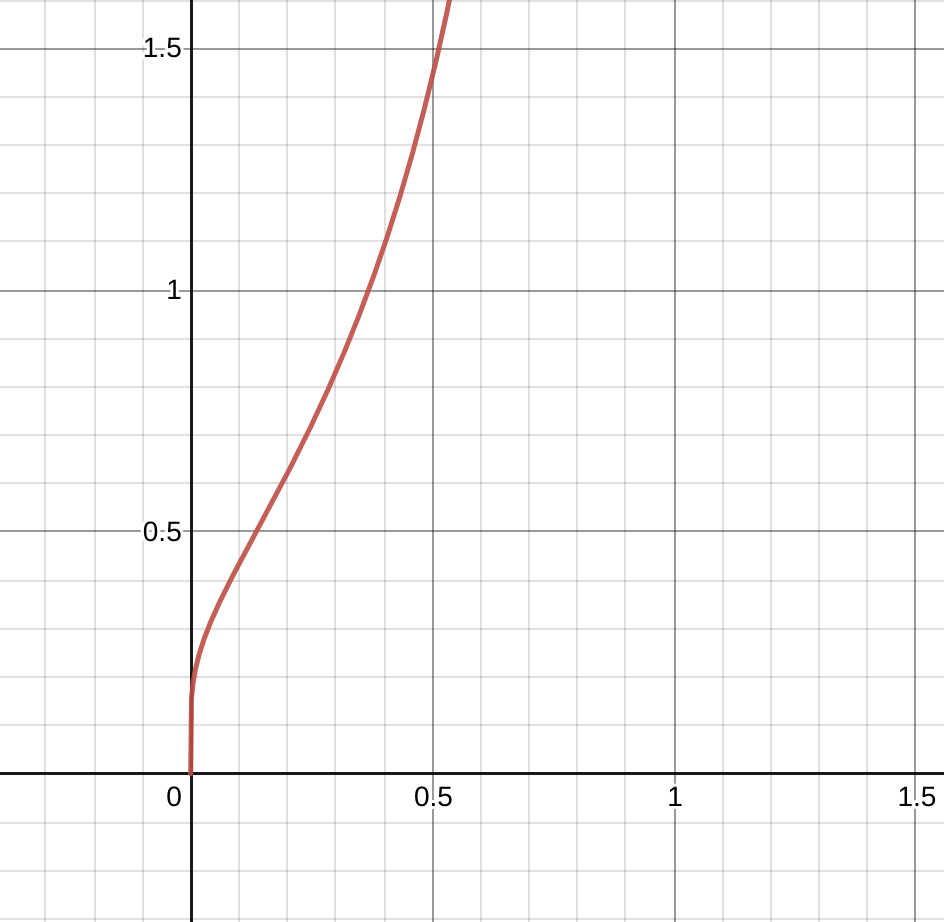
\includegraphics[width=\linewidth]{HMM_Only/function.png}
      \caption{}
      \label{func}
    \end{subfigure}
    \begin{subfigure}{.45\textwidth}
      \centering
      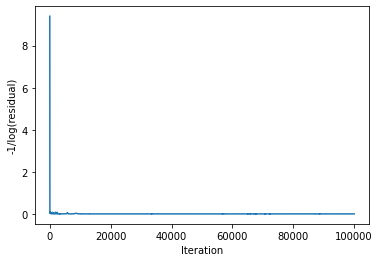
\includegraphics[width=\linewidth]{HMM_Only/convLog.png}
      \caption{}
      \label{convlog}
    \end{subfigure}
    \caption{}
\end{figure}

The values decrease quite rapidly, thus to create a visual representation we used the function $ y = \dfrac{-1}{ln(x)}$, where $x$ is the residual, to scale the values. We can see in Figure \ref{func} that our function is strictly increasing thus can be used for scaling. 

Along with the csv files containing the log, a graphical reprsentation can be found in the Analysis jupyter notebooks within each months folder. Figure \ref{convlog} shows one such graphical reprsentation for the covergence log of attempt 1 for month 0. We can see that the residual converges to 0 quite quickly, suggesting we could potentially reduce the number of iterations. The convergence itself confirms that the our two matrices and our intial distribution contain values close to the local optima. 





\subsection{Selecting the optimum optima}

As mentioned earlier, we perform multiple random starts to try and obtain the global optimum. However, from the model alone we do not know if it is the "most optimum". To do this we count frequencies. 

For each attempt we count and record the frequency of occurance of each interger in our observation set from our training rainfall data of 1000 observations as well as from our simulation generated by the HMM, also containing 1000 observations. We now find the difference the two sets of frequencies, square the given value and then take a sum. The attempt the lowest sum of squares is then accepted as the most optimum optima. 

For our example of month 0, we had the following results:
\begin{center}
  \begin{tabular}{c c}
    Attempt & Sum of Square difference \\
    1 & 656 \\
    2 & 672 \\
    3 & 1692
  \end{tabular}
\end{center}

As such we selected attempt 1 for our testing. The attempt selected for each month is given in below table.

\begin{center}
  \begin{tabular}{c c c c c c c c c c c c c}
    Month   &  0  & 1 & 2 & 3 & 4 & 5 & 6 & 7 & 8 & 9 & 10 & 11 \\
    Attempt &  1  & 3 & 2 & 1 & 1 & 1 & 1 & 2 & 2 & 3 & 3  & 2 
  \end{tabular}  
\end{center}

\subsection{Results}

Since the results for each month are quite similar , we will only present results for month 0. The Results for other months can be found in the analysis files accopymanying each months folder. 

\begin{figure}
    \begin{subfigure}{.45\textwidth}
      \centering
      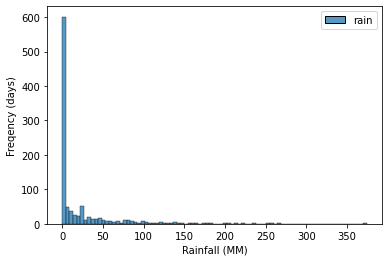
\includegraphics[width=\linewidth]{HMM_Only/0_freq_data.png}
      \caption{}
      \label{inc0:data}
    \end{subfigure}
    \begin{subfigure}{.45\textwidth}
      \centering
      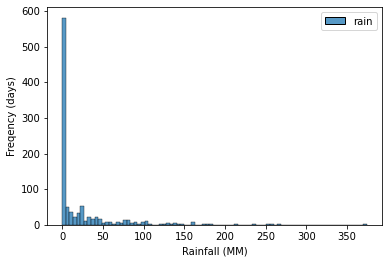
\includegraphics[width=\linewidth]{HMM_Only/0_freq_sim.png}
      \caption{}
      \label{inc0:sim}
    \end{subfigure}

    \begin{subfigure}{.45\textwidth}
      \centering
      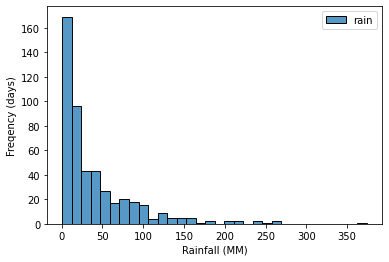
\includegraphics[width=\linewidth]{HMM_Only/_freq_data.png}
      \caption{}
      \label{inc0:n0data}
    \end{subfigure}
    \begin{subfigure}{.45\textwidth}
      \centering
      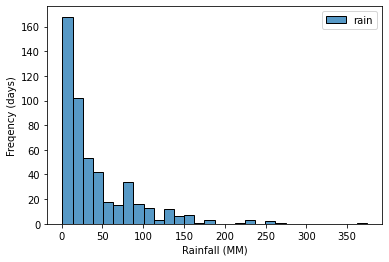
\includegraphics[width=\linewidth]{HMM_Only/_freq_sim.png}
      \caption{}
      \label{inc0:n0sim}
    \end{subfigure}
    \caption{}
    \label{inc0}
\end{figure}

From Figure \ref{inc0} we can see that the frequencies seem to be simliar for both simulation and recorded data. Furthermore, smaller details such as the peak at around 25mm also remains consitent. While this is promosing, the large frequency for 0mm distorts the graph. To compare further we plot the histograms once more, removing the first bar for 0mm. Here we can see it is not identical but seems to have similar properties, such as max, medium and high density areas. We will investigate this result numerically in the results chapter of this paper.


